\section{Bow shock data from Kobulnicky et al. (2016, 2017, 2018)}
\label{app:bow-shock-data}

In a series of papers \citet{Kobulnicky:2016a, Kobulnicky:2017a,
  Kobulnicky:2018a} provide an extensive mid-infrared-selected sample
of over 700 candidate stellar bow shock nebulae.  For 20 of these
sources, reliable distances and spectral classifications are provided
(Table~5 of \citealp{Kobulnicky:2017a} and 
\citealp{Kobulnicky:2018a}), and these are used in
\S~\ref{sec:summary-discussion}, where we discuss the
\(\tau\)--\(\eta\) diagnostic diagram.  In this appendix, we outline our
treatment and analysis of the data in these catalogs, which differs in
some important respects from that of the original authors.

The most important quantity to be derived from the observations is the
absorption optical depth, \(\tau\), of the bow shell to the stellar radiation.


\begin{figure}
  \centering
  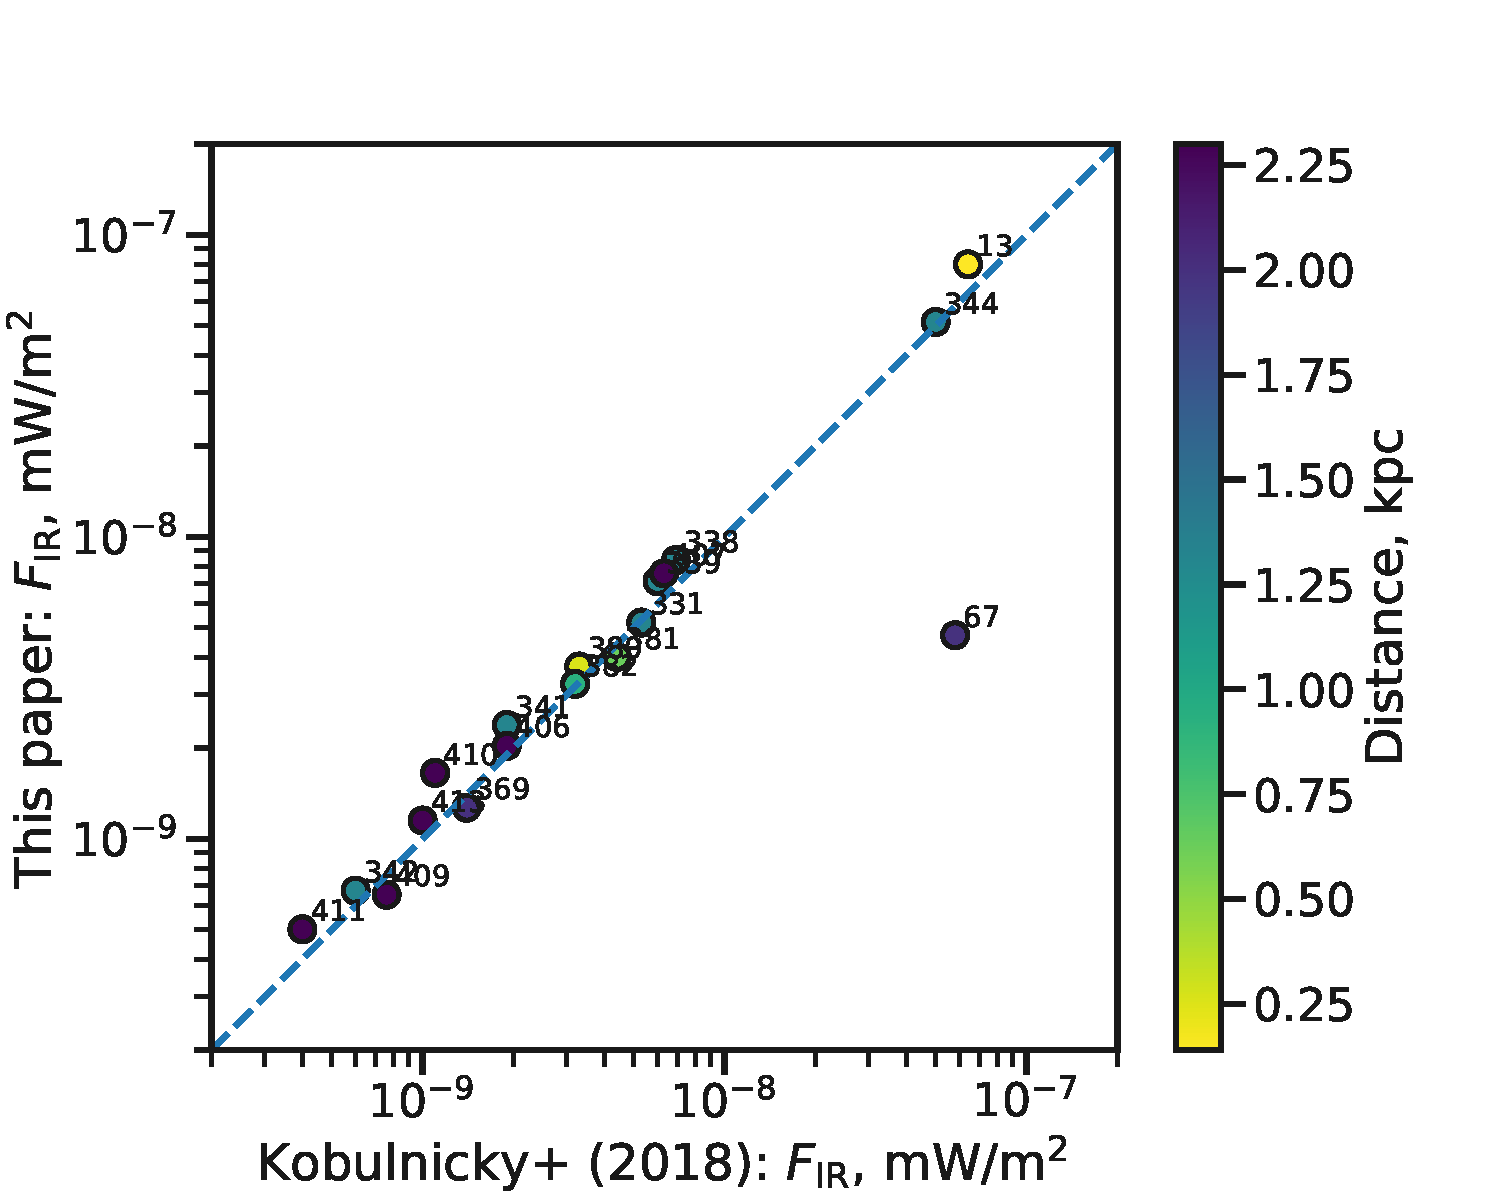
\includegraphics[width=\linewidth]{figs/K18-flux-comparison}
  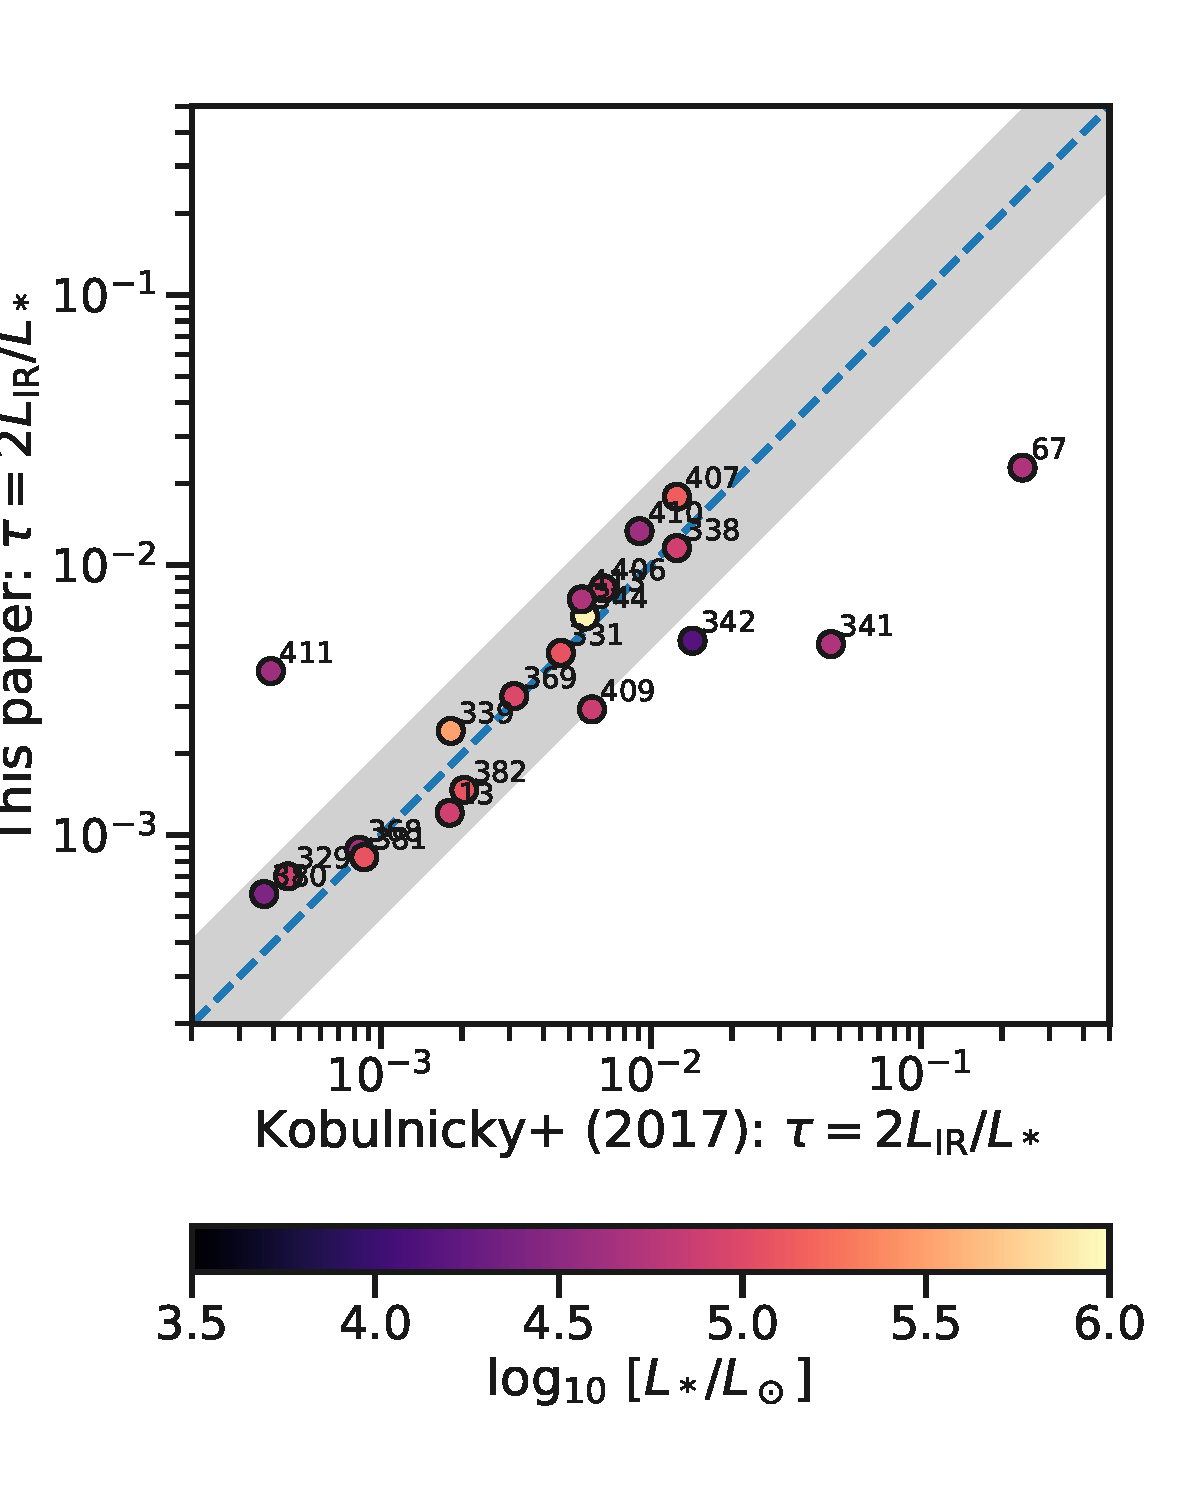
\includegraphics[width=\linewidth]{figs/K17-tau-comparison}
  \caption{Comparison}
  \label{fig:k17-k18-comparison}
\end{figure}

% So everything looks OK, except:

% * Source 67 is over 10 times too bright in the Kobulnicky table

% So, I will use my fluxes instead.  

\begin{figure*}
  \centering
  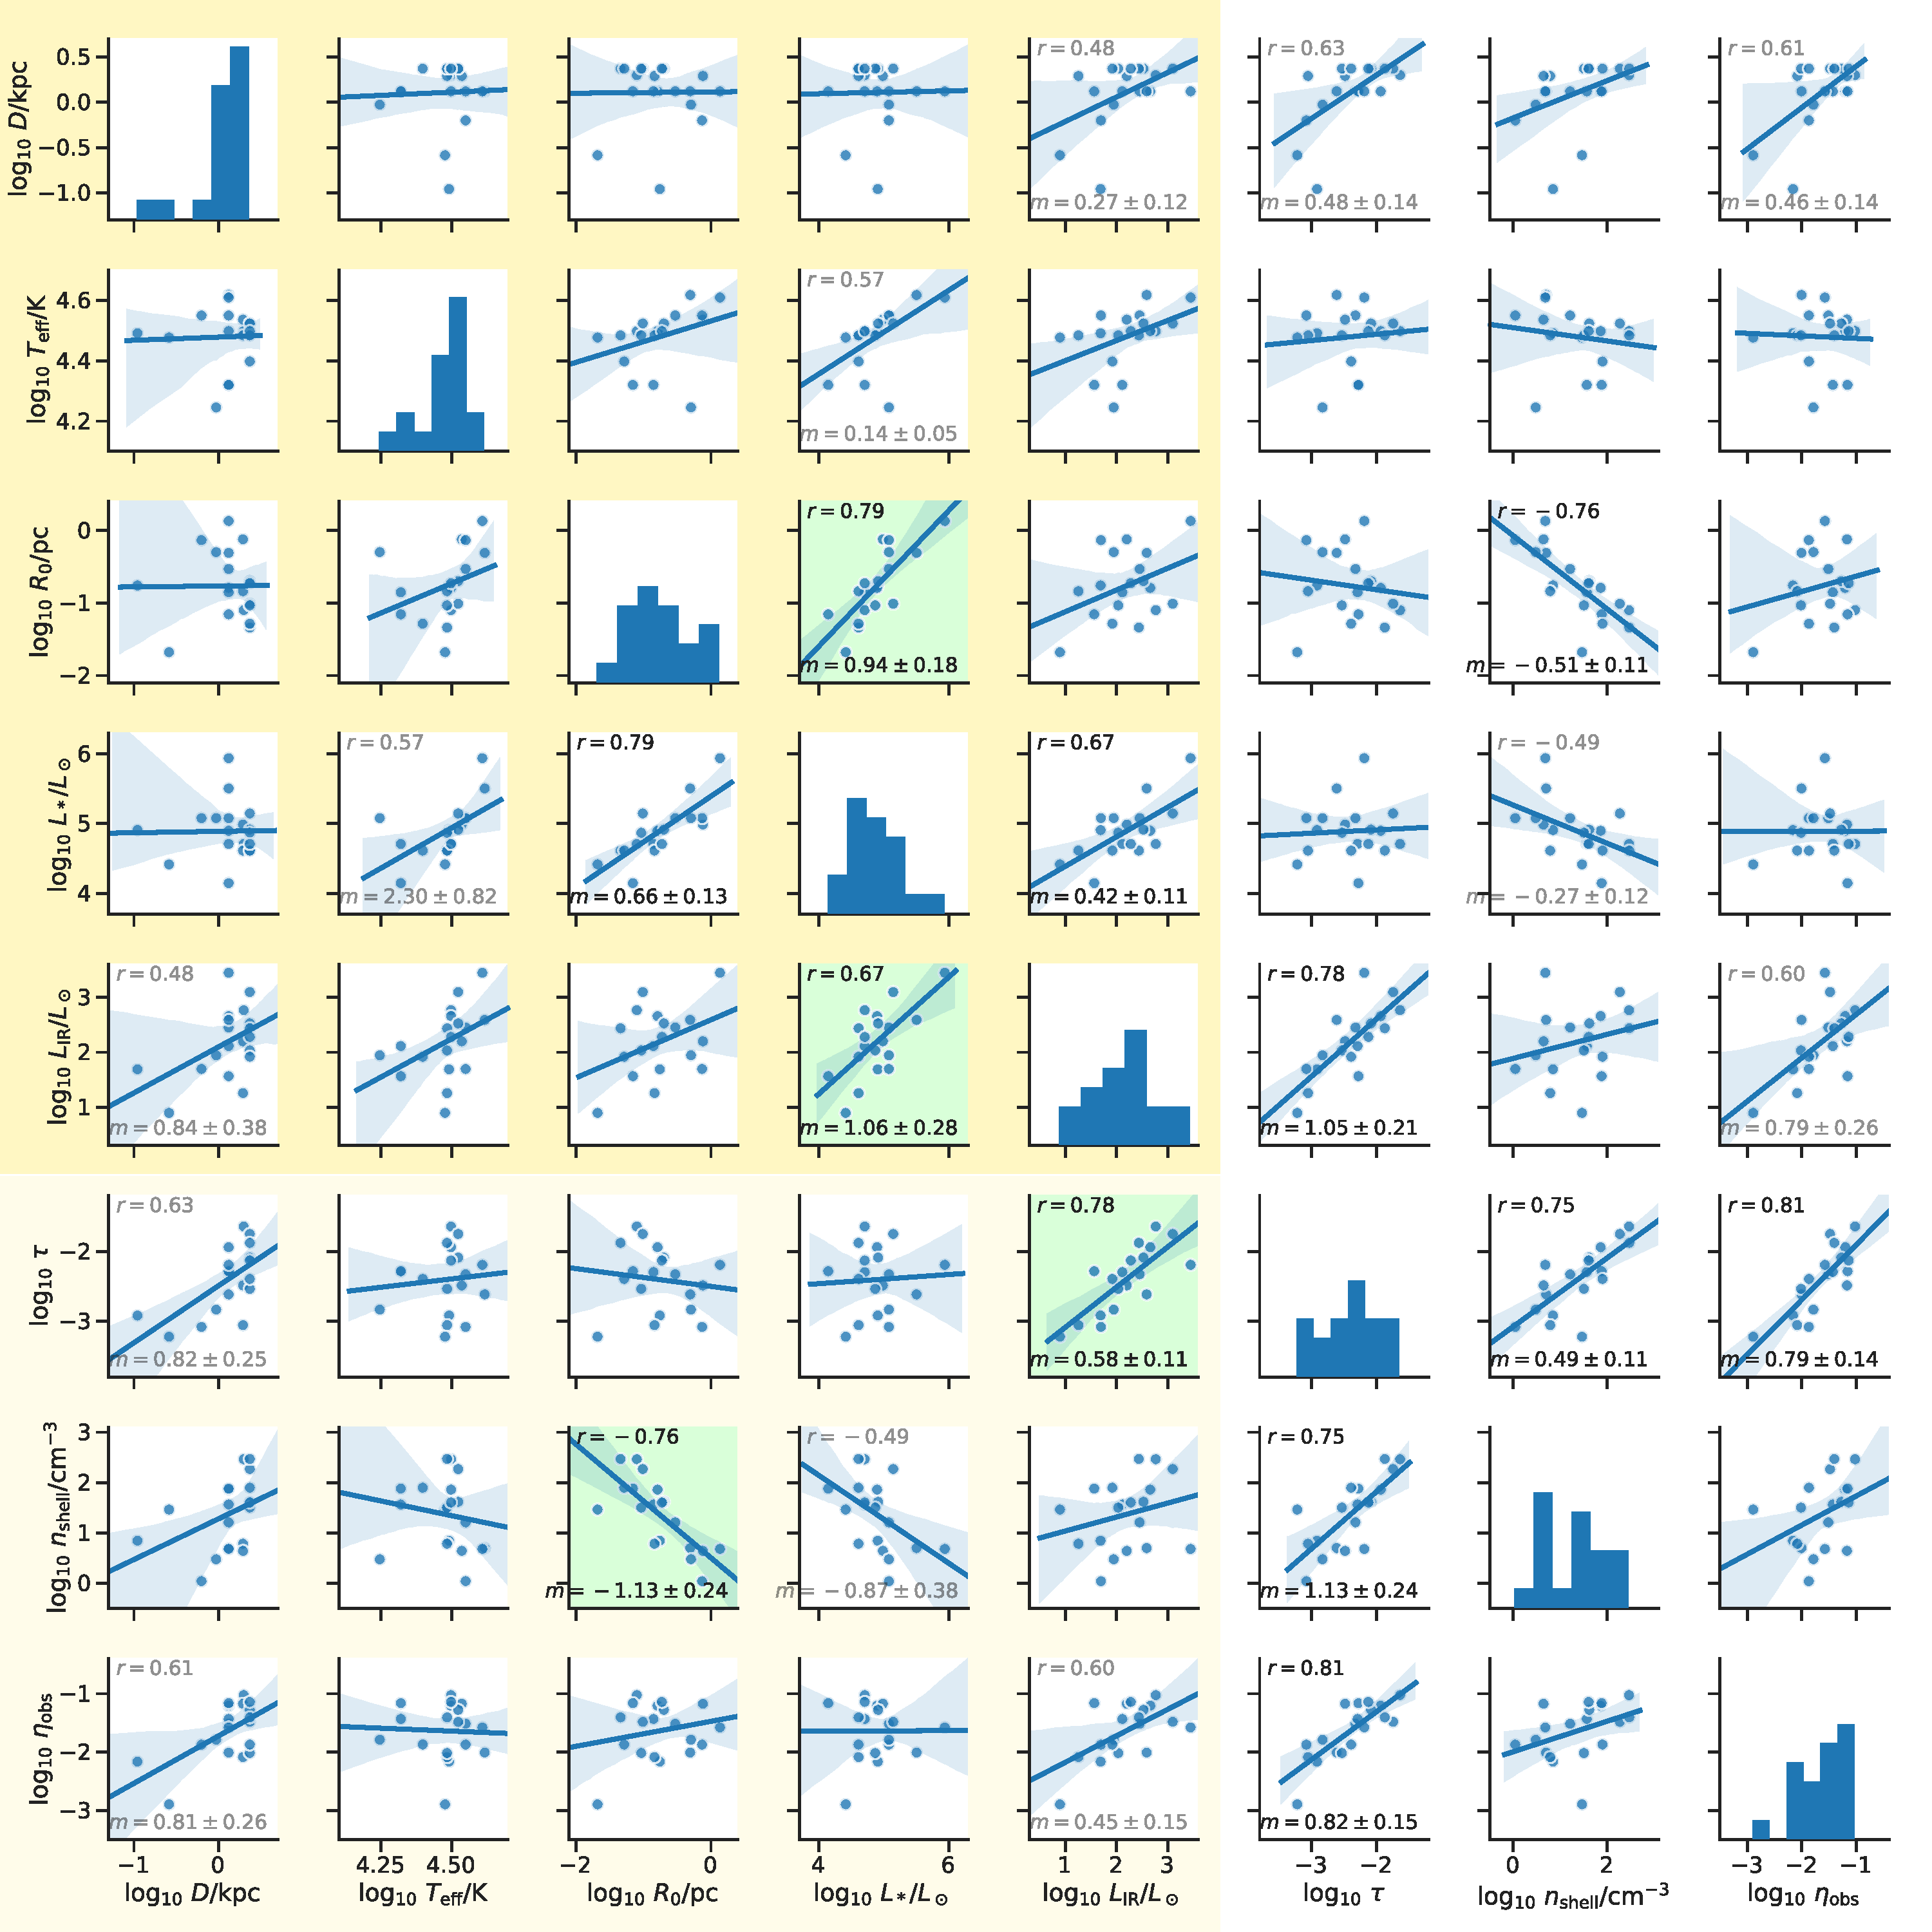
\includegraphics[width=\linewidth]{figs/K18-pairplot-edited}
  \caption[K18 pair plot]{Pair plots of correlations between observed
    and derived parameters of bows from the \citep{Kobulnicky:2018a}
    sample.}
  \label{fig:K18-pairplot-edited}
\end{figure*}


% In this graph we compare the original luminosity ratio taken directly from the Kobulnicky (2017) table (x axis) with the ratio calculated using my new total IR fluxes, combined with the new luminosities in the Kobulnicky (2018) table (y axis).   Most of the points show reasonable agreement between the two methods, with a few exceptions:

% * 67: this had the $F_\text{IR}$ overestimated in K17.  Using a more reasonable value gives a lower $\tau$
% * 341: The spectral class has changed from B2 (K17) to O9 (K18), increasing the assumed $L_*$, which lowers $\tau$
% * 411: The luminosity class has changed from Ib (K17) to V (K18), so $L_*$ has been greatly reduced, which increases the estimated $\tau$

% And there doesn't seem to be any significant correlation with stellar luminosity.

%%% Local Variables:
%%% mode: latex
%%% TeX-master: "dusty-bow-wave"
%%% End:
